\documentclass[12pt]{article}
\usepackage{times} % Make text more compressed.
\usepackage{url} % Allow URLs.
\usepackage{graphicx} % Allow inclusion of graphics.
\usepackage[sort&compress]{natbib} % Better bibliography handling.
\usepackage[margin=0.8in]{geometry} % Sets page size and margins
\usepackage{authblk} % Put authors names in a block.
\usepackage{amsmath} % Allow fancy math stuff
\usepackage{amsfonts}
\usepackage{tabularx,ragged2e,booktabs} % Stuff for tables.
\usepackage{titlesec}
\usepackage{amssymb}
\usepackage{comment}
\usepackage{subcaption}
\usepackage{authblk}
\usepackage{xcolor} % Allow colors.
\usepackage{hyperref}
\usepackage{amssymb}
\usepackage{dsfont}
\usepackage{float}
\usepackage[ruled,vlined]{algorithm2e}


\newcommand{\norm}[1]{\left\lVert#1\right\rVert}
\DeclareMathOperator*{\argmax}{arg\,max}
\DeclareMathOperator*{\argmin}{arg\,min}

% Use the short form for ISMB submission, long for biorxiv.
\newcommand{\shorten}[1]{#1}
%\newcommand{\shorten}[1]{}

\newcommand{\fixme}[2]{\color{red}{\bf #2 ---#1} \color{black}}
%\newcommand{\fixme}[2]{}

% Reduce the size of the affiliations
\renewcommand\Affilfont{\fontsize{9}{10.8}\itshape}

\title{Modelling Gene Expression by Integrating GRNs and HMs using GCNs}

\author[1,2]{Shalin Patel} 
\author[1,2,3]{TBD}
\author[2,3]{Ritambhara Singh}

\affil[1]{Division of Applied Mathematics, Brown University}
\affil[2]{Center for Computational Molecular Biology, Brown University}
\affil[3]{Department of Computer Science, Brown University}



\date{\vspace{-1.6cm}}

\begin{document}

\maketitle

\begin{abstract}

\end{abstract}

\section{Introduction}

\section{Related Work}

\section{Method}
\subsection{Formulation for Task} 
In this paper, we use the same inputs and outputs as Attentive and DeepChrome while also adding a gene expression matrix for each cell line. Using the same formulation as Cheng \emph{et al.} the task is formulated as measuring the gene expression as either up (1) or down (0) regulated. First, per cell line, a GRN is precomputed which utilizes a matrix $E$ of size $S\times G$ where $S$ denotes the number of samples in the expression matrix while $G$ represents the number of genes that were recorded. \\\\
Hence, for a sample gene, two pieces of information are fed. The first is $H$ which is a graph describing gene-gene interactions for a particular cell line. In the case of this paper $H$ was an adjacency list representation of the graph. Second, per gene, a matrix $X$ of size $M\times T$ was utilized where $M$ denotes the number of histone marks utilized while $T$ is the total number of bin positions taken into account around the TSS site of a gene. \\\\
Overall, for the training data of the GCN, we utilized $H$ and a $N\times M\times T$ sized matrix where $N$ is the number of gene samples. The output, accordingly, is a $N$-sized vector with either 0 or 1.

\subsection{Construction of GRNs}
The gene regulatory networks for this paper are built using the standard method of random forests. Utilizing the grnboost2 algorithm from the arboreto package on \url{pypi.org}, a regression task was defined for each gene in a cell line. \\\\
Let $E_i$ denote the row vector containing all samples for gene $i$ in the expression matrix. Then, specifically, for gene $i$, a random forest model $R_i$ was defined where, $L(R_i(E_{1:G\setminus i}), E_i)$ is minimized with $L$ denoting the mean square error. Once this task is completed, denote the set $\mathfrak{N}_i = \{imp(R_i, j) \mid j \in \{1:G\}\setminus i\}$. Here, $imp(R_i, j)$ refers to the feature importance of $j$ in random forest model $R_i$. Then the final graph $H$ is constructed with the neighbor list of a node $i$ being $\mathfrak{I}_i = \{j \mid imp(R_i, j) > \bar{\mathfrak{N}_i} + s(\mathfrak{N}_i)\}$ with $s(\mathfrak{N}_i)$ denoting the sample standard deviation. Hence, $H = \{\mathfrak{I}_i\}$, $\forall i$.
\section{Experimental Setup}

\section{Results}
\subsection{Performance Evaluation}
\begin{table}
    \centering
    \begin{tabular}{l || c | c | c | c | c | c | c || r}
        & E003 & E066 & E071 & E096 & E114 & E116 & E118 & \emph{Average}\\ \hline
        GCN & \textbf{0.7146} & \textbf{0.7503} & \textbf{0.6512} & \textbf{0.6883} & \textbf{0.7966} & 0.9168 & \textbf{0.8220} & \textbf{0.7628} \\
        Random & 0.4996 & 0.4968 & 0.6066 & 0.5000 & 0.6143 & 0.5032 & 0.5000 & \\
        Permute & 0.6899 & 0.6999 & 0.6125 & 0.6389 & 0.7527 & 0.8624 & 0.7649 & 0.7094 \\
        Attentive & 0.6759 & 0.7468 & 0.4906 & 0.5319 & 0.7930 & \textbf{0.9225} & 0.8181 & 0.7113 \\
        MLP & 0.6894 & 0.7035 & 0.6220 & 0.6420 & 0.7477 & 0.8606 & 0.7661 & 0.7188 
    \end{tabular}
    \caption{AUC Performance Evaluation Across Cell Lines and Baselines}
    \label{table:Table1}
\end{table}
\begin{figure}
    \centering
    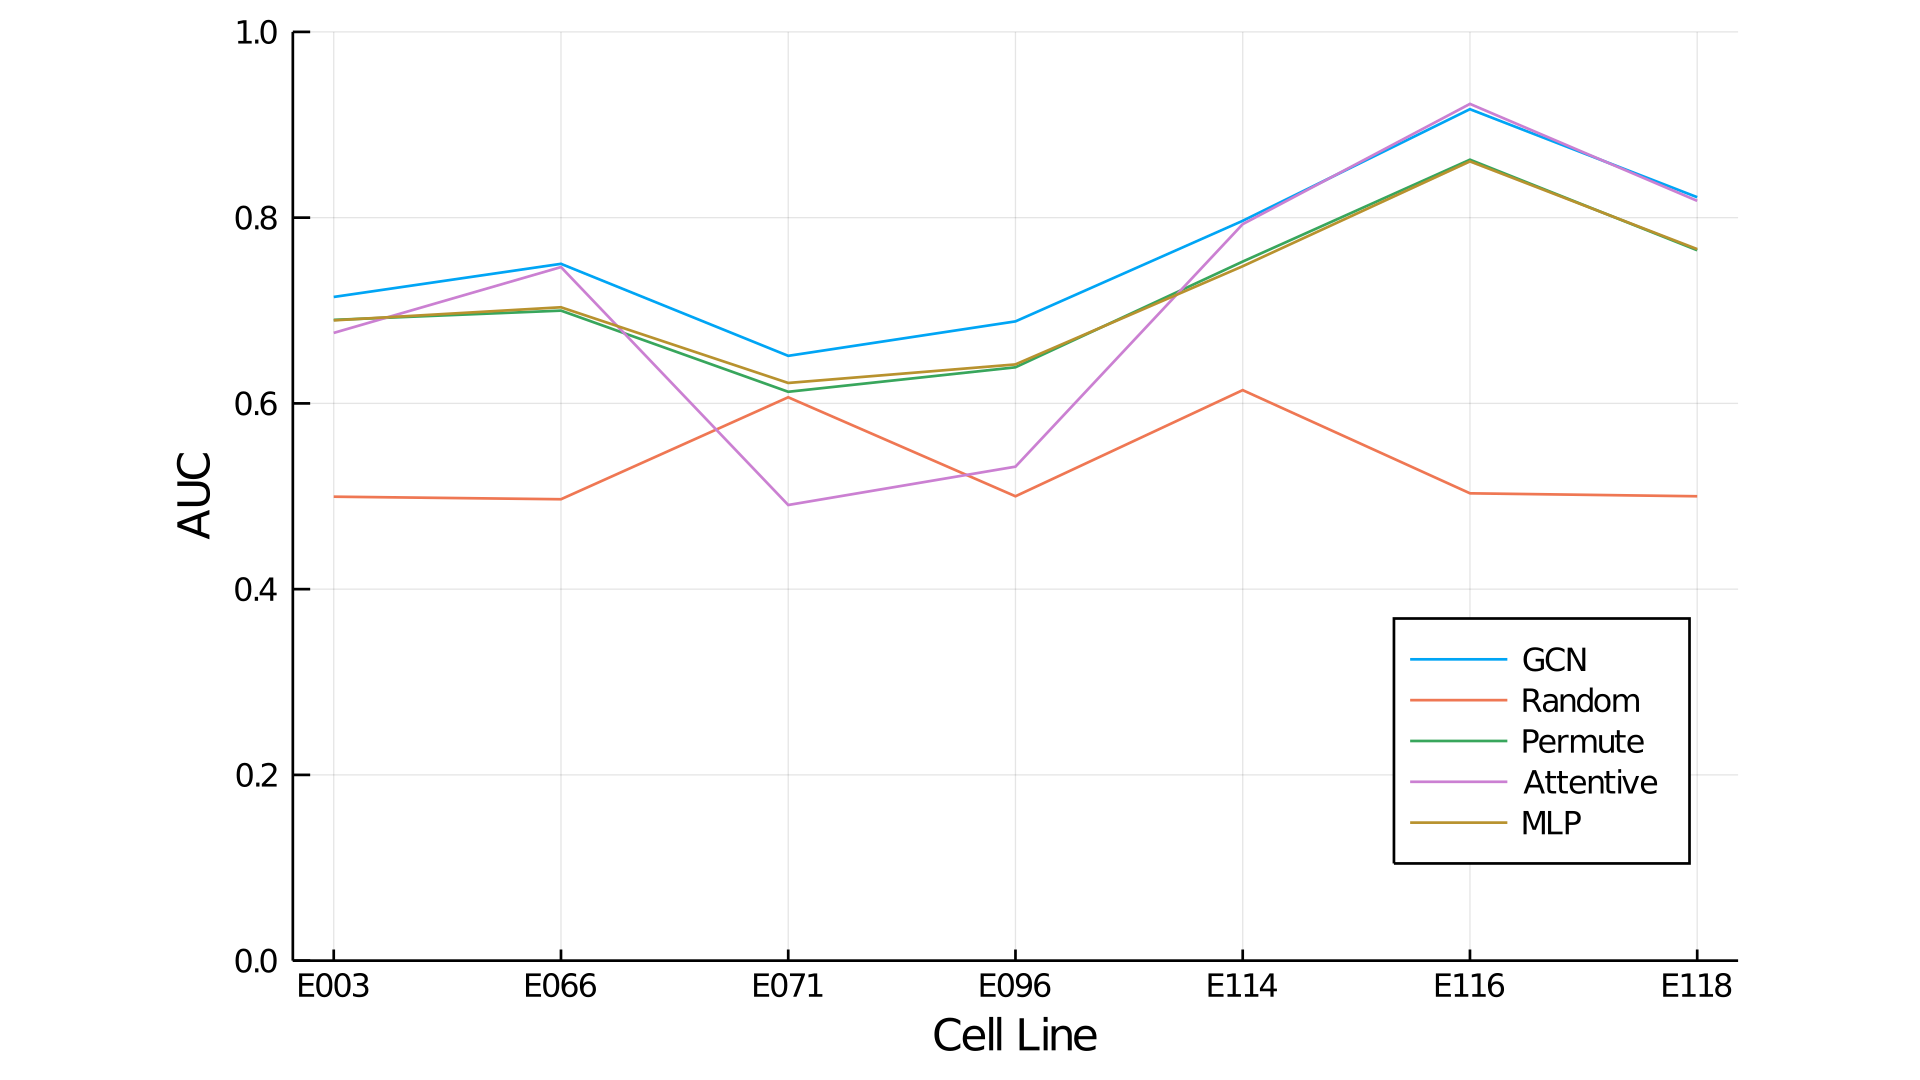
\includegraphics[width=\textwidth]{images/performance.png}
    \caption{AUC Performance Across Cell Lines and Baselines Method}
    \label{figure:Figure1}
\end{figure}
The performance of the model was checked against four baselines across seven different cell lines and is summarized in Table \ref{table:Table1}. \\\\
Quite clearly, the GCN model outperforms almost all of the other baseline methods, including the state of the art AttentiveChrome, across the cell lines. The only cell line where the GCN model was beaten was in the E116 cell line which was high performing across models. It is clear, though, that the GCN model shows great consistency and proves performance gains in lower performing cell lines such as E071. This is encapsulated in the average AUC performance metric across cell lines where the GCN model has a significantly higher average than all other models and in Figure \ref{figure:Figure1}. 

\section{Discussion}


\paragraph{Acknowledgments}.

\paragraph{Funding} 

\bibliographystyle{unsrt}
\small{\bibliography{refs}}
\end{document}



